\documentclass[a4paper,UKenglish]{lipics}

\usepackage{microtype}
%\usepackage[colorinlistoftodos]{todonotes} 
\usepackage{tikz}
\usepackage{latexsym}     
\usepackage{hyperref}
\usepackage{multicol}
\usepackage{stmaryrd}
\usepackage{amsmath}
\usepackage{amssymb}
\usepackage{url}
\usepackage{textcomp}
\usepackage{bussproofs}

\usetikzlibrary{shapes}                
\usetikzlibrary{fit}

\bibliographystyle{plain}
\pagestyle{headings}

\title{Verification of redecoration for infinite triangular matrices
  using coinduction}

\author[1]{Ralph Matthes}
\author[2]{Celia Picard}
\affil[1]{Institut de Recherche en Informatique de Toulouse (IRIT), \\
  C.N.R.S. and University of Toulouse, France}
\affil[2]{Institut de Recherche en Informatique de Toulouse (IRIT), \\
  University of Toulouse, France}
\authorrunning{ R. Matthes and C. Picard} 

\subjclass{F.3.1 Specifying and Verifying and Reasoning about Programs}
\keywords{nested datatype, coinduction, theorem proving, Coq}\Copyright[nc-nd]{R. Matthes and C. Picard}
%%% before exchange with the editor, we had
%%\Copyright[nc-nd] % or nd only!
%%\phantom{}
\serieslogo{}%
\volumeinfo%
     {Nils Anders Danielsson, Bengt Nordstr\"om}%
     {2}%
     {18th International Workshop on Types for Proofs and Programs (TYPES~2011)}%
     {19}%
     {1}%
     {57}%
   \EventShortName{TYPES 2011}
   \DOI{10.4230/LIPIcs.TYPES.2011.57}%


%%%%%%%%%%%%%%%%%%%%%%%%%%%%%%%%%%%%%%%%%%%%%%%%%%%%%%%
% Macros for references
%%%%%%%%%%%%%%%%%%%%%%%%%%%%%%%%%%%%%%%%%%%%%%%%%%%%%%%
\newcommand{\rdef}[1]{Definition~\ref{def:#1}}
\newcommand{\rlem}[1]{Lemma~\ref{lemma:#1}}
\newcommand{\rthm}[1]{Theorem~\ref{thm:#1}}
\newcommand{\rprop}[1]{Property~\ref{prop:#1}}
\newcommand{\rsect}[1]{Section~\ref{sect:#1}}
\newcommand{\rfig}[1]{Figure~\ref{fig:#1}}
\newcommand{\rcor}[1]{Corollary~\ref{cor:#1}}
\newcommand{\rex}[1]{Example~\ref{ex:#1}}
\newcommand{\rrem}[1]{Remark~\ref{rem:#1}}
%%%%%%%%%%%%%%%%%%%%%%%%%%%%%%%%%%%%%%%%%%%%%%%%%%%%%%%

%%%%%%%%%%%%%%%%%%%%%%%%%%%%%%%%%%%%%%%%%%%%%%%%%%%%%%%
% Macros for Tri
%%%%%%%%%%%%%%%%%%%%%%%%%%%%%%%%%%%%%%%%%%%%%%%%%%%%%%%
\newcommand{\Tri}{\ensuremath{\mathit{Tri}}}
\newcommand{\Trap}{\ensuremath{\mathit{Trap}}}
\newcommand{\pair}[2]{\langle #1,#2\rangle}
\newcommand{\redec}{\ensuremath{\mathit{redec}}}
\newcommand{\Rel}{\ensuremath{\mathit{Rel}}}
\newcommand{\Prop}{\ensuremath{\mathit{Prop}}}
\newcommand{\bisim}{\ensuremath{\mathbin{\simeq}}} %~~
\newcommand{\topT}{\ensuremath{\mathit{top}}}
\newcommand{\rest}{\ensuremath{\mathit{rest}}}
\newcommand{\cut}{\ensuremath{\mathit{cut}}}
\newcommand{\escut}{\ensuremath{\mathit{es\_cut}}}
\newcommand{\frow}{\ensuremath{\mathit{frow}}}
\newcommand{\constr}{\ensuremath{\mathit{constr}}}
\newcommand{\lift}{\ensuremath{\mathit{lift}}}
\newcommand{\fst}{\ensuremath{\mathit{fst}}}

\newcommand{\counit}{\ensuremath{\mathit{counit}}}
\newcommand{\cobind}{\ensuremath{\mathit{cobind}}}
\newcommand{\simcom}{\ensuremath{\mathbin{\approxeq}}} %~~^
\newcommand{\addes}{\ensuremath{\mathit{addes}}}
%%%%%%%%%%%%%%%%%%%%%%%%%%%%%%%%%%%%%%%%%%%%%%%%%%%%%%%

%%%%%%%%%%%%%%%%%%%%%%%%%%%%%%%%%%%%%%%%%%%%%%%%%%%%%%%
% Macros for Stream
%%%%%%%%%%%%%%%%%%%%%%%%%%%%%%%%%%%%%%%%%%%%%%%%%%%%%%%
\newcommand{\Str}{\ensuremath{\mathit{Str}}}
\newcommand{\EqSt}{\ensuremath{\mathbin{\equiv}}} %==
\newcommand{\map}{\ensuremath{\mathit{map}}}
\newcommand{\tl}{\ensuremath{\mathit{tl}}}
\newcommand{\hd}{\ensuremath{\mathit{hd}}}
\newcommand{\zipWith}{\ensuremath{\mathit{zipWith}}}
\newcommand{\es}{\ensuremath{\mathit{es}}}
%%%%%%%%%%%%%%%%%%%%%%%%%%%%%%%%%%%%%%%%%%%%%%%%%%%%%%%

%%%%%%%%%%%%%%%%%%%%%%%%%%%%%%%%%%%%%%%%%%%%%%%%%%%%%%%
% Macros for TriS
%%%%%%%%%%%%%%%%%%%%%%%%%%%%%%%%%%%%%%%%%%%%%%%%%%%%%%%
\newcommand{\vari}{'}%{^\star}
\newcommand{\TriS}{\ensuremath{\mathit{Tri\vari}}}
\newcommand{\tSR}{\ensuremath{\mathit{toStreamRep}}}
\newcommand{\fSR}{\ensuremath{\mathit{fromStreamRep}}}
\newcommand{\bisimS}{\ensuremath{\mathbin{\cong}}} %==^
\newcommand{\topS}{\ensuremath{\mathit{top\vari}}}
\newcommand{\frowS}{\ensuremath{\mathit{frow\vari}}}
\newcommand{\restS}{\ensuremath{\mathit{rest\vari}}}
\newcommand{\redecS}{\ensuremath{\mathit{redec\vari}}}
\newcommand{\liftS}{\ensuremath{\mathit{lift\vari}}}
\newcommand{\redecSG}{\ensuremath{\mathit{redec\vari_{gen}}}}
\newcommand{\redecSS}{\ensuremath{\mathit{redec\vari_{alt}}}}
\newcommand{\addesS}{\ensuremath{\mathit{addes\vari}}}
\newcommand{\tls}{\ensuremath{\mathit{tails}}}
%%%%%%%%%%%%%%%%%%%%%%%%%%%%%%%%%%%%%%%%%%%%%%%%%%%%%%%

%%%%%%%%%%%%%%%%%%%%%%%%%%%%%%%%%%%%%%%%%%%%%%%%%%%%%%%
% Macros for Tri_fin
%%%%%%%%%%%%%%%%%%%%%%%%%%%%%%%%%%%%%%%%%%%%%%%%%%%%%%%
\newcommand{\Trif}{\ensuremath{\mathit{Tri_{fin}}}}
\newcommand{\constrf}{\ensuremath{\mathit{constr_{fin}}}}
\newcommand{\sgf}{\ensuremath{\mathit{sg_{fin}}}}

%%%%%%%%%%%%%%%%%%%%%%%%%%%%%%%%%%%%%%%%%%%%%%%%%%%%%%%
% Macros for TriL
%%%%%%%%%%%%%%%%%%%%%%%%%%%%%%%%%%%%%%%%%%%%%%%%%%%%%%%
\newcommand{\cutL}{\ensuremath{\mathit{cutL}}}
\newcommand{\tLR}{\ensuremath{\mathit{toListRep}}}
\newcommand{\fLR}{\ensuremath{\mathit{fromListRep}}}
%%%%%%%%%%%%%%%%%%%%%%%%%%%%%%%%%%%%%%%%%%%%%%%%%%%%%%%


\begin{document}

\maketitle



\begin{abstract}
Finite triangular matrices with a dedicated type for the diagonal
elements can be profitably represented by a nested data type, i.\,e., a
heterogeneous family of inductive data types, while infinite
triangular matrices form an example of a nested coinductive type,
which is a heterogeneous family of coinductive data types. 

Redecoration for infinite triangular matrices is taken up from
previous work involving the first author, and it is shown that
redecoration forms a comonad with respect to bisimilarity.

The main result, however, is a validation of the original algorithm
against a model based on infinite streams of infinite streams. The
two formulations are even provably equivalent, and the second is
identified as a special instance of the generic cobind operation
resulting from the well-known comultiplication operation on streams
that creates the stream of successive tails of a given stream. Thus,
perhaps surprisingly, the verification of redecoration is easier for
infinite triangular matrices than for their finite counterpart.

All the results have been obtained and are fully formalized in the
current version of the Coq 
theorem proving environment where these coinductive datatypes are
fully supported since the version 8.1, released in 2007. 
Nonetheless, instead of displaying the Coq development, we have chosen
to write the paper in standard mathematical and type-theoretic 
language. Thus, it should be accessible without any specific knowledge about
Coq.

\end{abstract}
\section{Introduction}\label{sect:intro}
Redecoration for the finite
triangles has been verified against a list-based model in previous work
\cite{types07}. This is the point of departure for our present paper.

Finite triangles can be represented by ``triangular matrices'',
i.\,e., finite square matrices, where the part below the diagonal has
been cut off.  Equivalently, one may see them as symmetric matrices
where the redundant information below the diagonal has been
omitted. The elements on the diagonal play a different role than the
other elements in many mathematical applications, e.\,g., one might
require that the diagonal elements are invertible (non-zero). This is
modeled as follows: a type $E$ of elements outside the diagonal is
fixed throughout (we won't mention it as parameter of any of our
definitions), and there is a type of diagonal elements that enters all
definitions as an explicit parameter. More technically, if $A$ is the type of
diagonal elements, then $\Trif\,A$ shall denote the type of finite
triangular matrices with $A$'s on the diagonal and $E$'s outside (see
\rfig{visu_col}). Then, $\Trif$ becomes a family of types, indexed
over all types, hence a type transformation. Moreover, the different
$\Trif\,A$ are inductive datatypes that are all defined
simultaneously, hence they are an ``inductive family of types'' or
``\emph{nested datatype}'' \cite{birdmeertens}.

\begin{figure}[h]
  \centering
  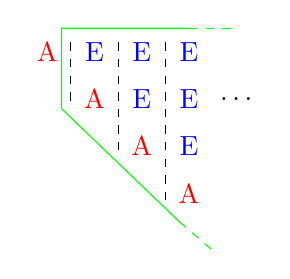
\begin{tikzpicture}[scale = 0.6]
    \foreach \y in {0,...,2}
    {\foreach \x in {\y,...,2}
      \draw (\x+1, -\y) node[color=blue]{E} ;
    }
    \foreach \x in {0,...,3} \draw (\x, -\x) node[color=red]{A} ;
    \draw(4,-1) node{$\ldots$};
    \draw[style = dashed](0.5,0.2) -- (0.5,-1.2);
    \draw[style = dashed](1.5,0.2) -- (1.5,-2.2);
    \draw[style = dashed, thin](2.5,0.2) -- (2.5,-3.2);
    
    \draw[color=green]  (3,0.5) -- (0.3,0.5) -- (0.3,
    -1.2)  -- (2.8,-3.6);
    \draw[color=green, dashed]  (3,0.5) -- (4,0.5);
    \draw[color=green, dashed]  (2.8,-3.6) -- (3.5,-4.2);
  \end{tikzpicture}\\[-2ex]
  \caption{Dividing a triangle into columns}
  \label{fig:visu_col}
\end{figure}

\vspace{-1ex}
If we cut the triangle into the first column and the rest, we get one
element of $A$ and a ``\emph{trapezium}'', with an uppermost row
solely consisting of $E$'s. In order not to have to ensure explicitly
by a dependent type that the number of columns is coherent, the
solution is to transform the trapezium into a triangle, integrating
the side diagonal (just above the diagonal) into the diagonal itself,
as shown in \rfig{tri_trap}.
From the left to the right, the lowermost element of $E$ in each
column is paired with the element of $A$ on the diagonal, and the
other elements of $E$ remain untouched.

\begin{figure}[h]
  \centering
  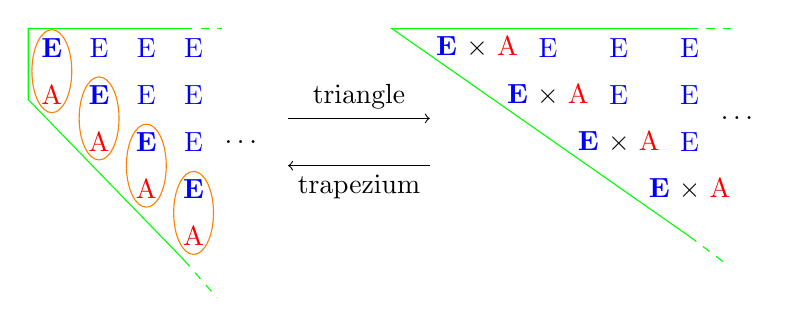
\begin{tikzpicture}[scale = 0.6]
    \foreach \y in {0,...,2}
    {\foreach \x in {\y,...,2}
      \draw (\x+1, -\y) node[color=blue]{E} ;
    }
    \foreach \x in {0,...,3} \draw (\x, -\x-1) node[color=red]{A} ;
    \foreach \x in {0,...,3} \draw (\x, -\x)
    node[color=blue]{\textbf{E}} ;
    \draw(4,-2) node{$\ldots$};

    \foreach \y in {0,...,2}
    {\foreach \x in {\y,...,2}
      \draw (1.5*\x+10.5, -\y) node[color=blue]{E} ;
    }
    \foreach \x in {0,...,3} \draw (1.5*\x+9, -\x)
    node{{\color{blue}\textbf{E}} $\times$ {\color{red} A}} ;
    \draw(14.5,-1.5) node{$\ldots$};
    
    \draw[->] (5,-1.5) to node[swap, auto, above]{triangle}
    (8,-1.5) ; 
    
    \draw[<-] (5,-2.5) to node[swap, auto, below]{trapezium}
    (8,-2.5) ; 

    \draw[color=green] (2.8,0.4) -- (-0.5,0.4) -- (-0.5, -1.1) --
    (2.8,-4.5)  ; 
    \draw[color=green, dashed] (2.8,0.4) -- (3.6,0.4) ; 
    \draw[color=green, dashed] (2.8,-4.5) -- (3.5,-5.3) ; 

    \draw[color=green] (13.5,0.4) -- (7.2,0.4) -- (13.5, -4); 
    \draw[color=green, dashed] (13.5,0.4) -- (14.4,0.4) ; 
    \draw[color=green, dashed] (13.5,-4) -- (14.3,-4.6) ; 

    \draw[color=orange](0, -0.5) ellipse (12pt and 25pt) ;  
    \draw[color=orange](1, -1.5) ellipse (12pt and 25pt) ;  
    \draw[color=orange](2, -2.5) ellipse (12pt and 25pt) ;  
    \draw[color=orange](3, -3.5) ellipse (12pt and 25pt) ;  
  \end{tikzpicture}\\[-2ex]
  \caption{}
  \label{fig:tri_trap}
\end{figure}

\vspace{-1ex}
Following this remark, the triangles can be defined
 theoretically \cite{grossestcspaper}, and in Coq and
Isabelle by the following constructors \cite{types07}:\\[-4ex]
\begin{multicols}{2}
  \begin{prooftree}
    \AxiomC {$a : A$}
    \UnaryInfC{$\sgf\,a : \Trif\,A$}
  \end{prooftree}
  \begin{prooftree}
    \AxiomC {$a : A$}
    \AxiomC {$t : \Trif(E\times A)$}
    \BinaryInfC{$\constrf\,a\,t : \Trif\,A$}
  \end{prooftree}
\end{multicols}

\vspace{-2.5ex}
\begin{remark}
  In this paper, single-lined inference rules denote 
  inductive definitions, double-lined inference rules are for
  coinductive definitions. 
\end{remark}

In more theoretical terms, \Trif{} is modeled as the \emph{least}
solution to the fixed-point equation
$$\Trif\,A=A+ A\times\Trif\,(E\times A)$$
The left summand corresponds to a triangle that only consists of a
single element of $A$ (a singleton), thus ensuring the base case.

The algorithm of redecoration (see work by Uustalu and Vene for
the general
categorical notion  \cite{DBLP:conf/sfp/UustaluV01}) is the following: for a given redecoration rule
$f:\Trif\,A\to B$, it is a function $\redec\,f$ that redecorates
$A$-triangles $t$ (elements of $\Trif\,A$) into $B$-triangles by
applying $f$ to the whole triangle $t$ to obtain the new top element,
and then by successively applying the same operation to the triangle
cut out from the remaining trapezium. This ends in the singleton case
where $f$ is applied to it and the result is turned into a triangle by
applying $\sgf$.  This algorithm only changes the diagonal elements in
$A$ into elements of $B$, as shown in \rfig{redecf}. We do not give
the formal definition of redecoration for finite triangles here.

\begin{figure}[h]
  \centering
  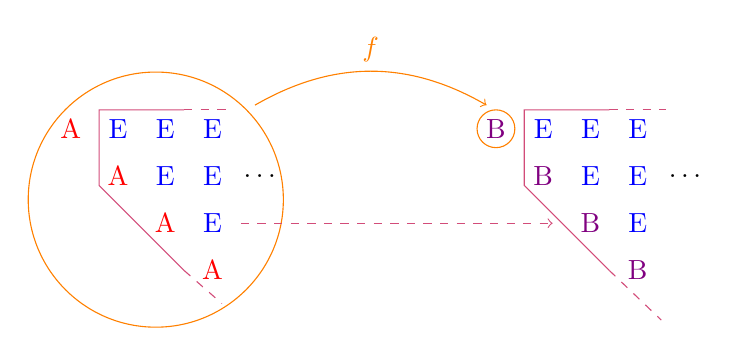
\begin{tikzpicture}[scale = 0.6]
    
    \foreach \y in {0,...,2}
    {\foreach \x in {\y,...,2}
      \draw (\x+1, -\y) node[color=blue]{E} ;
    }
    \foreach \x in {0,...,3} \draw (\x, -\x) node[color=red]{A} ;
    \draw(4,-1) node{$\ldots$};

    \foreach \y in {0,...,2}
    {\foreach \x in {\y,...,2}
      \draw (\x+10, -\y) node[color=blue]{E} ;
    }
    \foreach \x in {0,...,3} \draw (\x+9, -\x) node[color=violet]{B} ;
    \draw(13,-1) node{$\ldots$};
    \draw[color=purple!70]  (2.4, -3) --
    (0.6,-1.2) -- (0.6,0.4) -- (2.4,0.4);
    \draw[color=purple!70, dashed]  (2.4,0.4) -- (3.4,0.4);
    \draw[color=purple!70, dashed]  (2.4,-3) -- (3.2,-3.7);
 
    \draw[color=orange] (1.8,-1.5) circle(2.7cm);

    \draw[color=purple!70]  (11.4, -3) --
    (9.6,-1.2) -- (9.6,0.4) -- (11.4,0.4);
    \draw[color=purple!70, dashed]  (11.4,0.4) -- (12.6,0.4);
    \draw[color=purple!70, dashed]  (11.4,-3) -- (12.5,-4.05);
    
    \draw[color=orange] (9,0) circle(0.4cm);
    
    \draw[->,color = orange] (3.9,0.5) to [bend left] node[auto,
    swap, above]{$f$} (8.8,0.5) ; 

    \draw[->,color = purple!70, dashed] (3.6,-2) to (10.2,-2) ; 
    
  \end{tikzpicture}
  \caption{Redecoration}
  \label{fig:redecf}
\end{figure}

The redecoration for infinite
triangles \cite{grossestcspaper} has not yet been verified. This is
what we intend to do in this paper. 

Reasoning about nested coinductive types naturally rests on
observational equality, just as for ordinary coinductive types, and
since version 8.2, Coq greatly helps in using the rewrite mechanism
for Leibniz equality also for the notion of bisimilarity of infinite
triangular matrices.  With
respect to that notion of equality, redecoration is shown to form a
(sligthly weakened form of) comonad, and its implementation is
compared with an alternative one based on streams of streams.

These new results come with a full formalization in Coq \cite{TYPES11code}, and
limitations of what Coq recognizes as a guarded definition make the
theoretical development more challenging, but we still obtained smooth
results without an excessive overhead that would be imposed by a naive
dualization of the formalization for the finite triangles \cite{types07}.

In \rsect{original}, inspired by the previous theoretical development
\cite{grossestcspaper}, we introduce the dual to the definition of
finite triangles \cite{types07}. We present it with all the
tools necessary to define redecoration. We then propose a definition
for the redecoration algorithm on these infinite triangles and add
further tools and properties. In \rsect{streams}, we change the point
of view in the observation of the triangles. We give an alternative
definition for the infinite triangles, considering this new approach,
and provide various tools. We also show that this new representation
is equivalent to the previous one. Finally, we propose two ways of
defining redecoration, trying always to simplify and generalize our
definitions and show their adequation with previous definitions.

Since the results are fully formalized in the current version of Coq,
hence ensuring complete and sound proofs, we took the liberty to write the paper in
standard mathematical and type-theoretic language and also to omit
most proofs. Therefore, it should be accessible without any specific
knowledge about Coq. For the study of the development
\cite{TYPES11code}, the Coq'Art book \cite{coqart} should mostly suffice, but
the (type) class mechanism \cite{DBLP:conf/tphol/SozeauO08} and the
revised setoid rewriting mechanism based on it have to be consulted
elsewhere -- by default in the Coq Reference Manual \cite{MC}.


%%% Local Variables:
%%% mode: latex
%%% TeX-master: "coredec"
%%% End:

\section{Reference Representation with a Coinductive Family}\label{sect:original}

Dually to the representation of finite triangles discussed in the
introduction, ``triangular matrices'' are now introduced as
\emph{infinite} square matrices, where the part below the diagonal has
been cut off. Recall that a type $E$ of elements outside the diagonal
is fixed throughout. If $A$ is the type of diagonal elements, then
$\Tri\,A$ shall denote the type of infinite triangular matrices with
$A$'s on the diagonal and $E$'s outside. The different $\Tri\,A$ are
coinductive datatypes that are all defined simultaneously, as was the
case for \Trif{}, hence they are a ``coinductive family of types'' or
``\emph{nested codatatype}'', as will be developed below.

\subsection{Infinite triangles as nested coinductive type}

Infinite triangles can also be visualized as in \rfig{visu_col}, this time with the dots representing an infinite extension.



If we now cut the triangle into the first column and the rest, we get one
element of $A$ (as before for \Trif{}) and a trapezium, with an uppermost row
consisting of infinitely many $E$'s.

The $n$-th column consists of an element of $A$ on the diagonal and
$n$ elements of $E$ above the diagonal, as in the case of \Trif{}. As
before, we do not want to parameterize the type of the columns by
their index and instead integrate the side diagonal into the diagonal --
and this has to be done corecursively \cite{grossestcspaper}.
This integration is possible since trapeziums are again in one-to-one
correspondence to triangles, as shown in \rfig{tri_trap}, now interpreted infinitely.
In this figure, the trapezium to the left is considered as the
``trapezium view'' of the triangle to the right. Vice versa, the
triangle to the right is the ``triangle view'' of the trapezium to the
left.


We now formalize triangles through the following constructor that has to be interpreted coinductively.
\begin{definition}[$\Tri$, defined coinductively]\ 
    \begin{prooftree}
      \AxiomC {$a : A$}
      \AxiomC {$t : \Tri(E\times A)$}
      \doubleLine
      \BinaryInfC{$\constr\,a\,t : \Tri\,A$}
    \end{prooftree}
with $A$ a type variable.
\end{definition}


This means that the types $\Tri\,A$ for all types $A$ are simultaneously conceived as greatest solution to the fixed-point equation
$$Tri\,A = A \times \Tri(E\times A),$$
and \constr{} has two arguments instead of a pair of type $A\times\Tri(E\times A)$ just for technical convenience.

The second argument to \constr{} corresponds to the triangle view of the trapezium in our visualization in \rfig{visu_col}, but there
is no passage between a trapezium and a triangle -- this is only the motivation. In the formalization, there are only infinite triangles, but 
we set $\Trap\,A:=\Tri(E\times A)$ to hint to the trapezium view of these triangles.
\begin{definition}[Projections]\ 
  $$
  \begin{array}{l@{\hspace{2em}}l}
    \topT : \forall A.\,\Tri\,A \to A &
    \rest: \forall A.\, \Tri\,A \to \Trap\,A \\
    \topT\,(\constr\, a\, r) := a&
    \rest\,(\constr\, a\, r) := r
  \end{array}
  $$
\end{definition}
This definition by pattern matching implicitly uses the direction from
right to left in the above fixed-point equation. Thus, the top element and the trapezium part
of a triangle are calculated by unfolding the fixed point.

In order to obtain the triangle
that arises by cutting off the top row of a trapezium, we have to go
through all the columns.

\begin{definition}[$\cut:\forall A.\Trap\,A\to\Tri\,A$, defined corecursively]
$$\cut\,(\constr \,\pair e a\, r):=\constr\, a\,(\cut\, r)$$
\end{definition}

The definition does pattern matching on elements of $\Trap\,A$ and
constructs an element of the coinductive type $\Tri\,A$. The subterm
$\cut \,r$ represents a corecursive call to $\cut$, which is accepted
also by the Coq system as admissible corecursion since it is placed directly
as an argument to the constructor $\constr$.

\subsection{Redecoration for infinite triangles}

We are heading for a corecursive definition of the generic redecoration operation \redec{}
on triangles. It has type 
$$\forall A\forall B.\, (\Tri\,A\to B)\to\Tri\,A\to \Tri\,B,$$
which is the type of a coextension operation for $\Tri$ viewed as
support of a comonad.  Coextension -- also called cobind -- is the
dual of the extension / bind operation of a monad, which is so
successfully used in the functional programming language Haskell.
The counit for the comonad we are about to construct is our \topT{} operation.

Redecoration for \Tri{} follows the same pattern as for \Trif{}, but the successive applications of the same operation will never reach a base case, as there is none in \Tri{}. 


Formally, this is done by a corecursive definition, where
$\redec\,f\,t$ for $t$ of type $\Tri\,A$ has to call itself with
second argument of type $\Trap\,A$, hence $f$ is not even type-correct
as a first argument in that corecursive call. Instead of $f:\Tri\,A\to
B$, a ``lifted'' version of $f$ is needed that has type $\Tri(E\times
A)\to E\times B$.
\begin{definition}[$\lift:\forall A\forall B.\,(\Tri\,A\to B)\to \Tri(E\times A)\to E\times B$]
$$\lift\,f\,r:=\pair{\fst(\topT\,r)}{f(\cut\,r)}\enspace,$$
where $\fst$ is the first projection (from a pair to its first
component).  
\end{definition}
The definition is illustrated in \rfig{lift}.
\begin{figure}[h]
  \centering
  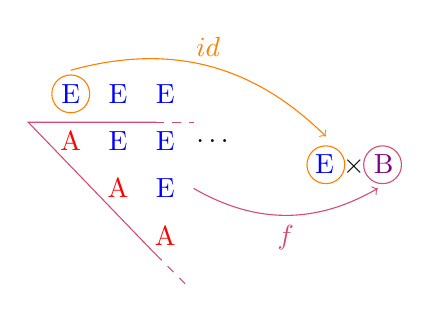
\begin{tikzpicture}[scale = 0.6]
    \foreach \y in {0,...,2}
    {\foreach \x in {\y,...,2}
      \draw (\x+1, -\y) node[color=blue]{E} ;
    }
    \foreach \x in {1,...,3} \draw (\x, -\x) node[color=red]{A} ;
    \draw(4,-1) node{$\ldots$};

     \draw (7,-1.5) node{{\color{blue} E} $\times$ {\color{violet} B}} ;
    \draw[color=orange] (1,0) circle(0.4cm);
    \draw[color=orange] (6.4,-1.5) circle(0.4cm);
    \draw[color=purple!70]  (2.8, -3.4) --
     (0.1,-0.6) -- (2.8,-0.6);
    \draw[color=purple!70, dashed]  (2.8,-0.6) -- (3.6,-0.6);
    \draw[color=purple!70, dashed]  (2.8,-3.4) -- (3.5,-4.1);

    \draw[color=purple!70] (7.6,-1.5) circle(0.4cm);

     \draw[->, color = orange] (1,0.5) to [bend left] node[auto,
     swap, above]{$id$} (6.4,-0.9) ; 
    \draw[->, color = purple!70] (3.6,-2) to [bend right] node[auto,
    swap, below]{$f$} (7.5,-2) ; 
    
  \end{tikzpicture}
  \vspace{-3ex}
  \caption{Definition of lifting}
  \label{fig:lift}
\end{figure}

The formal definition of redecoration is as follows:
\begin{definition}[$\redec:\forall A\forall B.\,(\Tri\,A\to B)\to \Tri\,A\to\Tri\,B$, defined corecursively]
$$\redec\,f\,t:=\constr\, (f\,t)\,\bigl(\redec\,(\lift\,f)\, (\rest\,t)\bigr)\enspace,$$
\end{definition}
see \rfig{redec}. 
This definition is accepted since it is guarded: the corecursive
call to $\redec$ is as second argument to $\constr$, and it does not
matter that the argument $f$ becomes $\lift\,f$ there. A function
argument that becomes more complicated in the recursive call is
typical of recursion on nested datatypes, see, e.\,g.,
\cite{grossestcspaper}.
\begin{figure}[h]
  \centering
  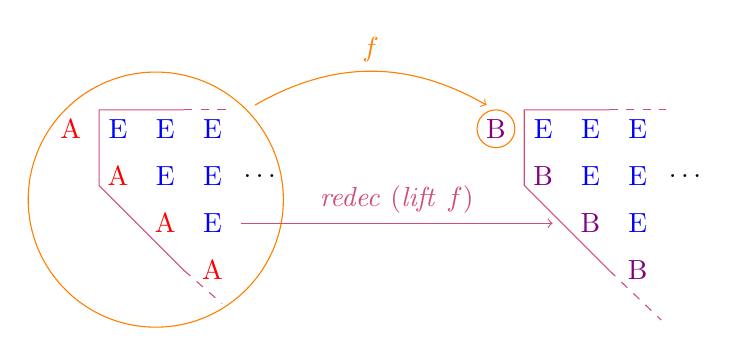
\begin{tikzpicture}[scale = 0.6]
    
    \foreach \y in {0,...,2}
    {\foreach \x in {\y,...,2}
      \draw (\x+1, -\y) node[color=blue]{E} ;
    }
    \foreach \x in {0,...,3} \draw (\x, -\x) node[color=red]{A} ;
    \draw(4,-1) node{$\ldots$};

    \foreach \y in {0,...,2}
    {\foreach \x in {\y,...,2}
      \draw (\x+10, -\y) node[color=blue]{E} ;
    }
    \foreach \x in {0,...,3} \draw (\x+9, -\x) node[color=violet]{B} ;
    \draw(13,-1) node{$\ldots$};
    \draw[color=purple!70]  (2.4, -3) --
    (0.6,-1.2) -- (0.6,0.4) -- (2.4,0.4);
    \draw[color=purple!70, dashed]  (2.4,0.4) -- (3.4,0.4);
    \draw[color=purple!70, dashed]  (2.4,-3) -- (3.2,-3.7);
 
    \draw[color=orange] (1.8,-1.5) circle(2.7cm);

    \draw[color=purple!70]  (11.4, -3) --
    (9.6,-1.2) -- (9.6,0.4) -- (11.4,0.4);
    \draw[color=purple!70, dashed]  (11.4,0.4) -- (12.6,0.4);
    \draw[color=purple!70, dashed]  (11.4,-3) -- (12.5,-4.05);
    
    \draw[color=orange] (9,0) circle(0.4cm);
    
    \draw[->,color = orange] (3.9,0.5) to [bend left] node[auto,
    swap, above]{$f$} (8.8,0.5) ; 

    \draw[->,color = purple!70] (3.6,-2) to node[auto,
    swap, above]{$\redec~(\lift~f)$} (10.2,-2) ; 
    
  \end{tikzpicture}
  \caption{Definition of redecoration}
  \label{fig:redec}
\end{figure}

This completes the definition, but leaves open the question if this is
really (in what sense) the cobind of a comonad and if it corresponds
to operations that are easier to understand than corecursion on nested
codatatypes. We note that recursion schemes for nested datatypes have
been subject of a long line of research, starting from work by Bird
and colleagues
\cite{birdmeertens,gfolds}.


\subsection{Properties of redecoration}

It is well-known that propositional equality $=$ (called Leibniz
equality in Coq since $t_1=t_2$ allows the replacement of $t_1$ by
$t_2$ in any mathematical context) cannot suffice as criterion for the
correctness of elements that are calculated in coinductive
types. Propositional equality cannot be established by coinductive
reasoning because this is confined to coinductively defined
conclusions, and propositional equality is not coinductive (in Coq, it
is defined inductively).  We write $\Rel\,C$ for the type of the
binary relations on $C$, and we use these relations in infix
notation. In Coq, their type is $C\to C\to\Prop$, where $\Prop$ is the
universe of propositions.

\begin{definition}[$\bisim:\forall A.\,\Rel(\Tri\,A)$, defined
  coinductively]\ 
        \begin{prooftree}
          \AxiomC {$t_1\,,\, t_2 : \Tri\,A$}
          \AxiomC {$\topT\,t_1 = \topT\,t_2$}
          \AxiomC {$\rest\,t_1\bisim\rest\,t_2$}
          \doubleLine
          \TrinaryInfC{$t_1\,\bisim\, t_2$}
        \end{prooftree}
\end{definition}
It is easy to show that \bisim{} is an equivalence relation for any
argument type $A$. It is an equivalence relation but not a congruence:
for every operation of interest we have to establish compatibility
with bisimilarity. This is in particular easily done for the
projection functions \topT{} and \rest{} and for the \cut{} operation.

Using this notion of bisimilarity, we can show that \redec{} is
extensional in its function argument (modulo \bisim{}), using full
extensionality of \lift{}:
\begin{lemma}\label{lemma:liftext}
  $\forall A \forall B \forall (f\, f': \Tri\,A \to B).\, 
  (\forall t, f\,t = f'\, t) \Rightarrow \forall t, \lift\,f\,t = \lift\,f'\, t$
\end{lemma}
\begin{lemma}
  $\forall A \forall B \forall (f\, f': \Tri\,A \to B).\, 
  (\forall t, f\,t = f'\, t) \Rightarrow \forall t, \redec\,f\,t \bisim \redec\,f'\, t$
\end{lemma}

The main properties of \redec{} we are interested in express that
\topT{} and \redec{} together constitute a comonad for ``functor''
\Tri{}.  The precise categorical definition in coextension form (with
a cobind operation instead of the traditional comultiplication) is,
e.\,g., given in \cite{DBLP:conf/sfp/UustaluV01}. Here, we give the
constructive notion we use in this paper, and it is parameterized by
an equivalence relation while classically, only mathematical equality
$=$ is employed.

\begin{definition}[Constructive comonad]
  A constructive comonad consists of a type transformation $T$, a
  function $\counit:\forall A.\,T\,A\to A$, a function
  $\cobind:\forall A\forall B.(T\,A\to B)\to T\,A\to T\,B$ and an
  equivalence relation $\simcom:\forall A.\,\Rel(T\,A)$ such that the
  following comonad laws hold:
\begin{eqnarray}
&&\forall A\forall B\forall f^{T\,A\to B}\forall t^{T\,A}.\, \counit (\cobind\,f\,t) = f\,t \\
&&\forall A\forall t^{T\,A}.\,\cobind\,\counit_A\,t \simcom t \\
&&\forall A\forall B\forall f^{T\, A \to B}\forall g^{T\, B \to C}\forall t^{T\, A}.\,\cobind\,(g \circ \cobind\,f)\,t \simcom\cobind\,g\,(\cobind\,f\,t)\label{thirdlaw}
  \end{eqnarray}
\end{definition}
Here, in order to save space, we gave the type information for the
term variables as superscripts. The index $A$ to \counit{} is meant to
say that the type parameter to \counit{} is set to $A$ -- in all other
cases, we leave type instantiation implicit.

\begin{definition}[Constructive weak comonad]
  A constructive weak comonad is defined as a constructive comonad,
  but where the equation in (\ref{thirdlaw}) is restricted to
  functions $g$ that are compatible with $\simcom$ in the following
  sense: $\forall t\,t', t \simcom t' \Rightarrow g\,t = g\,t'$.
\end{definition}

\begin{lemma}\label{lemma:TriWComonad}
  The type transformation \Tri{}, the projection function \topT{} and
  \redec{} form a constructive weak comonad with respect to \bisim{}.
\end{lemma}

The first comonad law is satisfied in an especially strong form:
$\topT(\redec\,f\,t)$ actually \emph{is} $f\,t$ by definition.  The
other comonad laws go through with suitable generalizations of the
lemmas -- in order to ensure guardedess of the proofs. The current
solution is unspectacular, but it was not obvious how to do it (much
more complicated solutions were found on the way and are now
obsolete). We only show the strengthening of the second comonad law,
but it is the same style for the third one.
\begin{lemma}[strengthened form of second comonad law for $\redec$]
  $$\forall A\forall (f:\Tri\,A\to A).\,(\forall (t:\Tri\,A), f\,t = \topT\,t) \Rightarrow \forall (t:\Tri\,A).\,\redec\,f\,t\bisim t$$
\end{lemma}
The proof is by coinduction and uses \rlem{liftext}. Obviously, this
implies the second comonad law.  For all the details, see our
formalization in Coq
\cite{TYPES11code}. We only get a weak comonad because proving
pointwise equality of $\lift (g \circ (\redec\,f))$ and $(\lift\, g)
\circ (\redec (\lift\,f))$ requires compatibility of $g$ with
\bisim{}, and this is a crucial step for proving the third comonad
law.

\medskip
When defining the \cut{} operation, one might naturally want to get also
the part that has been cut out (the elements of $E$). 
These elements are given by the following function:
\begin{definition}[$\escut : \forall A.\, \Trap\,A \to \Str\,E$, defined corecursively]
  $$\escut\,(\constr\,\pair e a\, r) := e :: (\escut\,r)$$
\end{definition}
\begin{remark}
  In the standard library of Coq, the type of streams with elements in type $C$ are predefined, and we can represent this definition as follows:
  \begin{prooftree}
    \AxiomC {$c : C$}
    \AxiomC {$s: \Str\,C$}
    \doubleLine
    \BinaryInfC{$c :: s : \Str\,C$}
  \end{prooftree}
  The projection functions are called \hd{} and \tl{}. They are such
  that $\hd(c :: s) = c$ and $\tl(c :: s) = s$. 
  We will also use the \map{} function defined by $\map\,f\,(c :: s) =
  f\,c :: (\map\,f\,s)$.
  
\end{remark}
Using \escut{}, we can define the first row of $E$ elements in a triangle as
$$\frow:\forall A.\,\Tri\,A\to\Str\,E\qquad\qquad\frow\,t:=\escut\,(\rest\,t)$$


Once we have these definitions, we might want to be able to ``glue''
the two cut parts in order to recreate the original trapezium. This is
done by the function \addes{}
\begin{definition}[$\addes : \forall A.\, \Str\,E \to \Tri\,A \to
  \Trap\, A$, defined corecursively]
  $$\addes\,(e :: \es)\,(\constr\, a\, r) := \constr\,\pair{e}{a}\,(\addes\,\es\,r)$$
\end{definition}
And it is then easy to show that \addes{} indeed performs the gluing:
$$ \forall A\forall(r:\Trap\,A).\, \addes\,(\escut\,r)\,(\cut\,r) \bisim r$$

%%% Local Variables:
%%% mode: latex
%%% TeX-master: "coredec"
%%% End:

\section{Another Conception of Triangles}\label{sect:streams}
In this section, we show another way to perceive and represent
infinite triangles. And we propose two ways of defining redecoration
on this new representation. 

\subsection{A new definition using streams}
In the previous section, we always visualized the infinite triangles
by their columns. Indeed, we said that a triangle was a first column
with only one element of type $A$ (the element of the diagonal) and a
trapezium, itself actually a triangle, as suggested in
\rfig{visu_col}. 

While elements of the finite triangles in $\Trif\,A$ (see
\rsect{intro}) are (globally) finite, also all the columns of our
infinite triangles in $\Tri\,A$ are finite. In the work that we
started from for this article \cite{types07},
redecoration on $\Trif$ is verified against a model where triangles
are represented by finite lists of columns, where each column consists
of the diagonal element in $A$ and a finite list of elements in $E$. A
naive dualization of that approach would consist in taking as
representation of infinite triangles streams of columns that would be
formed as for the finite ones. This mixture of inductive and
coinductive datatypes is notoriously difficult to handle. We have been
confronted with this problem many times in the last few years, as can
be seen in the second author's thesis \cite{theseCP} which deals with this kind of problems
particularly in Coq. But in other proof assistants, the same kind of
issues has appeared; there is also an experimental solution in Agda \cite{dan, daal}.  Still, the representation of infinite
triangles mixing inductive and coinductive datatypes can be carried
out, but we refrain from presenting this column-based approach here.

However, we can also visualize triangles the other way around. We now consider
the triangle by its rows, as suggested in \rfig{visu_row}.  
\begin{figure}[h]
  \centering
  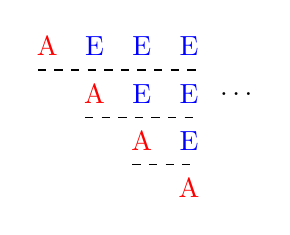
\begin{tikzpicture}[scale = 0.6]
    \foreach \y in {0,...,2}
    {\foreach \x in {\y,...,2}
      \draw (\x+1, -\y) node[color=blue]{E} ;
    }
    \foreach \x in {0,...,3} \draw (\x, -\x) node[color=red]{A} ;
    \draw(4,-1) node{$\ldots$};
    \draw[style = dashed](-0.2,-0.5) -- (3.2,-0.5);
    \draw[style = dashed](0.8,-1.5) -- (3.2,-1.5);
    \draw[style = dashed](1.8,-2.5) -- (3.2,-2.5);
  \end{tikzpicture}
  \vspace{-3ex}
  \caption{Dividing a triangle into rows}
  \label{fig:visu_row}
\end{figure}
Then, on any row, we have one element of type $A$ and infinitely many
elements of type $E$. And we also have infinitely many rows. Here,
nothing is finite (only the single element of $A$ at the head of each
row, but this is not a problem), therefore, we do not have any
embedded inductive type in our description -- unlike in the columnwise
decomposition mentioned above. This new visualization can be
represented as a stream of pairs made of one element of type $A$ and a
stream of elements of type $E$.

\begin{definition}
  $\TriS\,A := \Str (A \times \Str\,E)$
\end{definition}
Actually, following the definition of \Str{}, we can read this new definition of the triangles as
consisting of three parts: the top element, the stream of elements of
$E$ of the first row and the triangle corresponding to the rest, as
shown in \rfig{3elems}.
\begin{figure}[h]
  \centering
  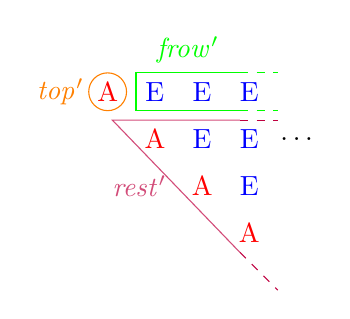
\begin{tikzpicture}[scale = 0.6]
    \foreach \y in {0,...,2}
    {\foreach \x in {\y,...,2}
      \draw (\x+1, -\y) node[color=blue]{E} ;
    }
    \foreach \x in {0,...,3} \draw (\x, -\x) node[color=red]{A} ;
    \draw(4,-1) node{$\ldots$};
    \draw[color=orange] (0,0) circle(0.4cm);
    \draw[color=orange] (-1,0) node{$\topS$};

    \draw[color=green] (2.8,0.4) -- node[auto, swap, above]{\frowS} (0.6,0.4) --
    (0.6,-0.4) -- (2.8,-0.4);
    \draw[color=purple!70]  (2.8,-0.6) --  (0.1,-0.6) -- node[auto, swap,
    left]{\restS}(2.8, -3.4);
     \draw[color=green, style = dashed](2.8,0.4) -- (3.6,0.4);
     \draw[color=green, style = dashed](2.8,-0.4) -- (3.6,-0.4);
     \draw[color=purple, style = dashed](2.8,-0.6) -- (3.6,-0.6);
     \draw[color=purple, style = dashed](2.8,-3.4) -- (3.6,-4.2);
  \end{tikzpicture}
  \vspace{-3ex}
  \caption{Conceptualizing a triangle as a triple}
  \label{fig:3elems}
\end{figure}

\noindent
We define functions that allow us to access to each of these elements: 
\begin{definition}[Projections]\ 
  $$
  \begin{array}{l@{\hspace{2em}}l@{\hspace{2em}}l}
    \topS : \forall A.\,\TriS\,A \to A &
    \frowS : \forall A.\, \TriS\,A \to \Str\,E &
    \restS: \forall A.\, \TriS\,A \to \TriS\,A \\
    \topS\,(\pair{a}{\es} :: t) := a&
    \frowS\,(\pair{a}{\es} :: t) := \es&
    \restS\,(\pair{a}{\es} :: t) := t
  \end{array}
  $$
\end{definition}
Notice that $\rest$ and $\restS$ are conceptually different -- the
former yields the trapeziums after cutting off the first column, the
latter triangles after cutting off the first row.

To compare two elements of \TriS{}, we need a notion of bisimilarity, which on \Str{} is pre-defined in
Coq as follows:
\begin{definition}[$\EqSt:\forall C.\,\Rel(\Str\,C)$, defined
  coinductively]\ 
        \begin{prooftree}
          \AxiomC {$s_1\,,\, s_2 : \Str\,C$}
          \AxiomC {$\hd\,s_1 = \hd\,s_2$}
          \AxiomC {$\tl\,s_1\EqSt\tl\,s_2$}
          \doubleLine
          \TrinaryInfC{$s_1\,\EqSt\, s_2$}
        \end{prooftree}
\end{definition}

However, we cannot use it directly. Indeed, we would need to prove,
for two triangles $t_1$ and $t_2$ that their first rows are
Leibniz-equal, i.\,e., $\frowS\,t_1 = \frowS\,t_2$. This is too
strict, since the rows are defined partially coinductively (because of
the stream of $E$'s). Therefore, we need to define a new relation on
\TriS{} that will compare the three elements of the triangles. The
tops can be compared through Leibniz equality, the first rows can be
compared using \EqSt{} and the rests with the relation on \TriS,
corecursively.
\begin{definition}[$\bisimS:\forall A.\,\Rel(\TriS\,A)$, defined
  coinductively]\label{lemma:bisimS}\ 
  \begin{prooftree}
    \AxiomC {$t_1\,,\, t_2 : \TriS\,A \hspace{5ex} \topS\,t_1 = \topS\,t_2$}
    \AxiomC {$\frowS\,t_1\EqSt\frowS\,t_2$}
    \AxiomC {$\restS\,t_1 \bisimS \restS\,t_2$}
    \doubleLine
    \TrinaryInfC{$t_1\,\bisimS\, t_2$}
  \end{prooftree}
\end{definition}
It is immediate to show that \bisimS{} is an equivalence relation. 

In order to validate this view of the triangles, we want to show that
it is indeed equivalent to the original one. Therefore, we are going
to show that there is a bijection between the two definitions (modulo
pointwise bisimilarity). To do so we define two conversion functions
(\tSR{}, from \Tri{} to \TriS{} and \fSR{} for the other way around) and show that their
compositions are pointwise bisimilar to the identity.

The two conversion functions are quite natural. To transform an
element of $\Tri\,A$ into an element of $\TriS\,A$, we need to reconstruct from
the original triangle the three elements of $\TriS\,A$. The top remains
the original top, this is trivial. The first row of elements of $E$ is given by \frow. Finally,
the triangle has to be transformed again by \tSR{} from the rest of
the triangle with the first row cut out by the function \cut. The
calculation for the different parts is represented in \rfig{tSR}. 
\begin{figure}[h]
  \centering
  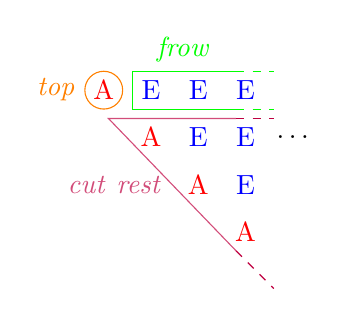
\begin{tikzpicture}[scale = 0.6]
    \foreach \y in {0,...,2}
    {\foreach \x in {\y,...,2}
      \draw (\x+1, -\y) node[color=blue]{E} ;
    }
    \foreach \x in {0,...,3} \draw (\x, -\x) node[color=red]{A} ;
    \draw(4,-1) node{$\ldots$};
    \draw[color=orange] (0,0) circle(0.4cm);
    \draw[color=orange] (-1,0) node{$\topT$};

    \draw[color=green] (2.8,0.4) -- node[auto, swap, above]{\frow} (0.6,0.4) --
    (0.6,-0.4) -- (2.8,-0.4);
    \draw[color=purple!70]  (2.8,-0.6) --  (0.1,-0.6) -- node[auto, swap,
    left]{\cut~\rest}(2.8, -3.4);
     \draw[color=green, style = dashed](2.8,0.4) -- (3.6,0.4);
     \draw[color=green, style = dashed](2.8,-0.4) -- (3.6,-0.4);
     \draw[color=purple, style = dashed](2.8,-0.6) -- (3.6,-0.6);
     \draw[color=purple, style = dashed](2.8,-3.4) -- (3.6,-4.2);
  \end{tikzpicture}
  \vspace{-3ex}
  \caption{Definition of \tSR}
  \label{fig:tSR}
\end{figure}
\begin{definition}[$\tSR: \forall A.\, \Tri\,A \to \TriS\,A$, defined corecursively]\label{def:tSR}
  $$\tSR\,t := \pair{\topT\,t}{\frow\,t} :: \tSR \,(\cut\, (\rest\,t))$$
\end{definition}
The definition of \fSR{} is also quite intuitive. We have to construct
the two elements that compose elements of type \Tri{}. The top remains
the top as before, this is again trivial. For the rest, we have to ``glue''
the first row to the rest of the triangle (basically the inverse of
the \cut{} and \escut{} functions on \TriS) before transforming it
again. 
We call \addesS{} the function that performs this operation, as shown
in \rfig{addesS}. 
\begin{figure}[h]
  \centering
  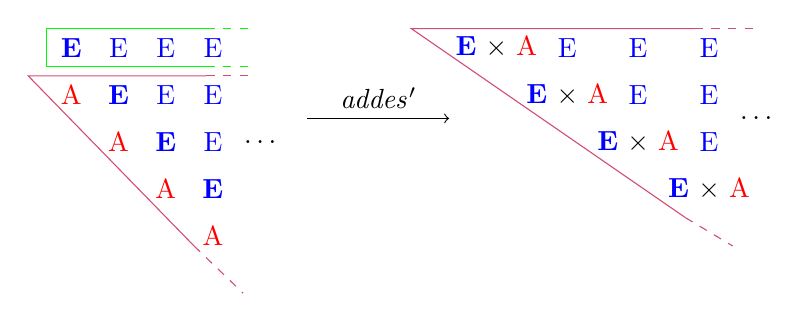
\begin{tikzpicture}[scale = 0.6]

    \foreach \y in {0,...,2}
    {\foreach \x in {\y,...,2}
      \draw (\x+1, -\y) node[color=blue]{E} ;
    }
    \foreach \x in {0,...,3} \draw (\x, -\x-1) node[color=red]{A} ;
    \foreach \x in {0,...,3} \draw (\x, -\x)
    node[color=blue]{\textbf{E}} ;
    \draw(4,-2) node{$\ldots$};

    \foreach \y in {0,...,2}
    {\foreach \x in {\y,...,2}
      \draw (1.5*\x+10.5, -\y) node[color=blue]{E} ;
    }
    \foreach \x in {0,...,3} \draw (1.5*\x+9, -\x)
    node{{\color{blue}\textbf{E}} $\times$ {\color{red} A}} ;
    \draw(14.5,-1.5) node{$\ldots$};
    
    \draw[->] (5,-1.5) to node[swap, auto, above]{\addesS}
    (8,-1.5) ; 

     \draw[color=green] (2.2*1.3,0.4) -- (-0.4*1.3,0.4) -- 
     (-0.4*1.3,-0.4) -- (2.2*1.3,-0.4);
     \draw[color=purple!70] (2.2*1.3,-0.6) -- (-0.7*1.3,-0.6) --
     (2*1.3, -4.2) ; 
     \draw[color=green, dashed] (2.2*1.3,0.4) -- (3*1.3,0.4);
     \draw[color=green, dashed] (2.2*1.3,-0.4) -- (3*1.3,-0.4);
     \draw[color=purple!70, dashed] (2.2*1.3,-0.6) -- (3*1.3,-0.6);
     \draw[color=purple!70, dashed] (2*1.3,-4.2) -- (2.8*1.3,-5.2);

     \draw[color=purple!70] (13.2,0.4) -- (7.2,0.4) -- (13, -3.6); 
     \draw[color=purple!70, dashed] (13.2,0.4) -- (14.5,0.4);
     \draw[color=purple!70, dashed] (13,-3.6) -- (14,-4.2);
    
  \end{tikzpicture}
  \caption{Definition of \addesS}
  \label{fig:addesS}
\end{figure}
\begin{definition}[$\addesS: \forall A.\, \Str\,E \to \TriS\,A \to \TriS
  (E\times A)$, defined corecursively]\label{def:addesS}
  $$\addesS\,(e :: \es)\,t := \pair{\pair{e}{\topS\,t}}{\es} :: \addesS\,(\frowS\,t)\,(\restS\,t)$$
\end{definition}
\begin{definition}[$\fSR: \forall A.\, \TriS\,A \to \Tri\,A$, defined corecursively]\label{def:fSR}
  $$\fSR\,t := \constr\,(\topS\,t)\,\bigl(\fSR\,(\addesS\,(\frowS\,t)\,(\restS\,t))\bigr)$$
\end{definition}
\begin{remark}
  Our first idea was to do the gluing after the
  transformation. Indeed, as the transformation does not affect the
  elements of $E$, it seemed more natural to us not to submit this
  part to the corecursive call of the transformation.
  Thus, we wanted to define \fSR{} coinductively as follows:
  $$ \fSR\,t := \constr\,(\topS\,t)\,(\addes\,(\frowS\,t)\,(\fSR\,
  (\restS\,t)))$$
  However, even if this seems harmless, this definition cannot be
  accepted by Coq since the corecursive call to \fSR{} is not
  guarded (it is an argument of \addes{} and not of a constructor). Nevertheless, we have shown that the solution to the
  previous equation is unique with respect to pointwise bisimilarity and that
  \fSR{} of \rdef{fSR} satisfies it. 
\end{remark}
\begin{lemma}\label{lemma:tSR_fSR}
  $\forall A\forall(t:\TriS\,A).\, \tSR\, (\fSR\,t) \bisimS t$
\end{lemma}
\begin{proof}
  To prove this result, we actually prove the following stronger
  result that we then only instantiate to finish the proof: 
  $$\forall A\forall (t:\TriS\,A)(u:\Tri\,A),\, \tSR \,(\fSR\,t) \bisimS u \Rightarrow t \bisimS u $$
  The proof of this statement is a simple coinduction, that uses some
  straightforward results on \cut{} and \addesS{}. 
\end{proof}
\begin{lemma}\label{lemma:fSR_tSR}
  $\forall A\forall (t:\Tri\,A).\, \fSR\, (\tSR\,t) \bisim t$
\end{lemma}
\begin{proof}
  We use the same technique as before. We prove a stronger result that
  we instiantiate to prove our lemma: 
  $$\forall A\forall (t:\Tri\,A)(u:\TriS\,A).\, \fSR\, (\tSR\,t) \bisim u \Rightarrow t \bisim u $$
  Here again, the proof is a straightforward coinduction using
  compatibility of \topT{} and \rest{} with $\bisim$ and a simple result on \addesS.
\end{proof}

\subsection{Redecoration on \TriS{}}
Thus, we have a completely different view of the triangles, but still,
it is fully equivalent to the original one.  The interest of this view
is that now the redecoration is very easy to perform. Indeed, before,
the tricky part was that we had to lift the function $f$ to
trapeziums, and therefore to cut out the elements of $E$ remaining
(implicitly) from the first row. The problem was that we roughly had to
cut out a row, while we were reasoning on columns. Here, as we
directly reason on rows, it is much easier. As shown in \rfig{redecS},
the three elements of the transformed triangle will be:
\begin{itemize}
  \item the top is the application of $f$ to the whole triangle (as before)
  \item the first row of elements of $E$ is  the same row as in the original
    triangle (and as we said we have direct access to it)
  \item the rest of the triangle is the application of the redecoration
    function to the rest
\end{itemize}

\begin{figure}[h]
  \centering
  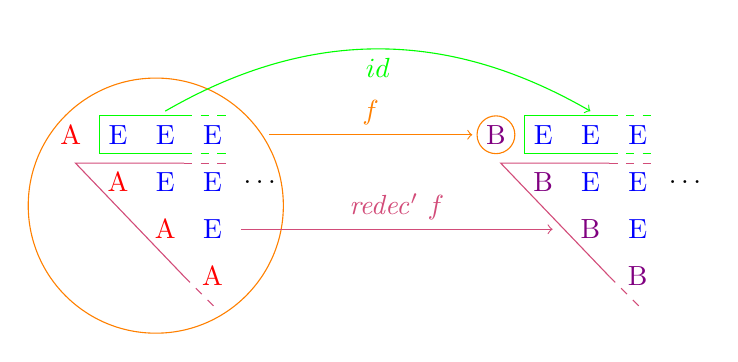
\begin{tikzpicture}[scale = 0.6]
    
    \foreach \y in {0,...,2}
    {\foreach \x in {\y,...,2}
      \draw (\x+1, -\y) node[color=blue]{E} ;
    }
    \foreach \x in {0,...,3} \draw (\x, -\x) node[color=red]{A} ;
    \draw(4,-1) node{$\ldots$};

    \foreach \y in {0,...,2}
    {\foreach \x in {\y,...,2}
      \draw (\x+10, -\y) node[color=blue]{E} ;
    }
    \foreach \x in {0,...,3} \draw (\x+9, -\x) node[color=violet]{B} ;
    \draw(13,-1) node{$\ldots$};
    \draw[color=purple!70]  (2.4, -3) --
    (0.1,-0.6) --  (2.4,-0.6);
    \draw[color=purple!70, dashed]  (2.4,-0.6) -- (3.4,-0.6);
    \draw[color=purple!70, dashed]  (2.4,-3) -- (3.1,-3.7);
 
    \draw[color=orange] (1.8,-1.5) circle(2.7cm);

    \draw[color=purple!70]  (11.4, -3) --
    (9.1,-0.6)-- (11.4,-0.6);
    \draw[color=purple!70, dashed]  (11.4,-0.6) -- (12.4,-0.6);
    \draw[color=purple!70, dashed]  (11.4,-3) -- (12.1,-3.7);
    
    \draw[color=orange] (9,0) circle(0.4cm);
    
    \draw[->,color = orange] (4.2,0) to node[auto,
    swap, above]{$f$} (8.5,0) ; 

    \draw[->,color = purple!70] (3.6,-2) to  node[auto,
    swap, above]{$\redecS~f$} (10.2,-2) ;
    \draw[->,color = green] (2,0.5) to [bend left] node[auto,
    swap, below]{$id$} (11,0.5) ;  


    \draw[color=green] (2.4,0.4) --  (0.6,0.4) -- 
    (0.6,-0.4) -- (2.4,-0.4);
    \draw[color=green, dashed]  (2.4,0.4) -- (3.4,0.4);
    \draw[color=green, dashed]  (2.4,-0.4) -- (3.4,-0.4);

    \draw[color=green] (11.4,0.4) --  (9.6,0.4) -- 
    (9.6,-0.4) -- (11.4,-0.4);
    \draw[color=green, dashed]  (11.4,0.4) -- (12.4,0.4);
    \draw[color=green, dashed]  (11.4,-0.4) -- (12.4,-0.4);

  \end{tikzpicture}
  \caption{Definition of redecoration}
  \label{fig:redecS}
\end{figure}

\noindent
Therefore, we can define the redecoration function for \TriS{} as
follows: 
\begin{definition}[$\redecS: \forall A\forall B.\,(\TriS\,A\to B)\to \TriS\,A\to\TriS\,B$, defined corecursively]\label{def:redecS}
  $$\redecS\,f\,t := \pair{f\,t}{\frowS\,t} :: \redecS\,f\,(\restS\,t)$$
\end{definition}
We can finally show that this new version of the redecoration is
equivalent to the previous one, modulo compatibility, using the conversion functions. We
show that:
\begin{lemma}\label{lemma:redecS_redec}
  $$
  \begin{array}{rl}
    \forall f, &
    (\forall t\,t', t \bisimS t' \Rightarrow f\,t = f\,t') \\
    \Rightarrow &
    \forall t, \redecS\,f\,t \bisimS \tSR\,(\redec\,(f \circ
    \tSR)\,(\fSR\,t)) 
  \end{array}
  $$ 
\end{lemma}
\begin{lemma}\label{lemma:redec_redecS}
  $$
  \begin{array}{rl}
    \forall f, &
    (\forall t\,t', t \bisim t' \Rightarrow f\,t = f\,t') \\
    \Rightarrow & \forall t, \redec\,f\,t \bisim \fSR\,(\redecS\,(f \circ
    \fSR)\,(\tSR\,t)) 
  \end{array}
  $$
\end{lemma}
\begin{remark}
  The compatibility hypotheses here are needed to work with \Tri{}. Up
  to these extra requirements, the two conversion functions yield an
  isomorphism of comonads (the associated properties for \topT{} and
  \topS{} are immediate by definition).
\end{remark}


\subsection{Simplifying redecoration again}

As the representation of infinite triangles \TriS{} is only as a stream
of streams, we can use standard functions on streams to define
redecoration. Indeed, redecoration can be interpreted as
consisting of applying a function to each element of the diagonal of
an infinite triangle, where each element of the diagonal is itself a
triangle (iterated tails of the given triangle). We can thus decompose the
redecoration operation into two steps: first transform the infinite
triangle into a triangle of triangles and then apply the
transformation function on the elements of the diagonal, as shown in
\rfig{redecS'_id}.
\begin{figure}[h]
  \centering
  \begin{tikzpicture}[scale = 0.6]
    
    \foreach \y in {0,...,2}
    {\foreach \x in {\y,...,2}
      \draw (\x+1, -\y-2) node[color=blue]{E} ;
    }
    \foreach \x in {0,...,3} \draw (\x, -\x-2) node[color=red]{A} ;
    \draw(4,-3) node{$\ldots$};


    \foreach \y in {0,...,2}
    {\foreach \x in {\y,...,2}
      \draw (1.7*\x+9.5, -2*\y-1) node[color=blue]{E} ;
    }
    
    
    \foreach \x in {0,...,2} 
    {
      
      \foreach \b in {0,...,\x}
      {\foreach \a in {0,...,\b}
        \draw (7.5+\b*0.5+4-\x*2, -\a*0.5-4+\x*2) node[color=orange,scale=0.6]{E} ;
      }
      \foreach \a in {\x,...,3} \draw (1.5*\x+7+\a*0.5, -\a*0.5-\x*1.5) node[color=orange,scale=0.6]{A} ;
      \draw(1.5*2-1.5*\x+9,-4.3+\x*1.8) node[color=orange, scale=0.5]{$\ldots$};
      
    }
    \draw (12.8,-6) node[color=orange, scale=0.6]{A};
    \draw (13.2,-6) node[color=orange, scale=0.5]{$\ldots$};
    \draw(14,-3) node{$\ldots$};

    \foreach \y in {0,...,2}
    {\foreach \x in {\y,...,2}
      \draw (\x+19, -\y-2) node[color=blue]{E} ;
    }
    \foreach \x in {0,...,3} \draw (\x+18, -\x-2) node[color=violet]{B} ;
    \draw(22,-3) node{$\ldots$};

    \draw[->,color = purple!80] (4.8,-3) to node[auto,
    swap, below]{$1^{\textrm{st}}$ step} (8.5,-3) ; 
    \draw[->,color = purple!80] (14.8,-3) to node[auto,
    swap, below]{$2^{\textrm{nd}}$ step} (18.5,-3) ; 

  \end{tikzpicture}
  \vspace{-1ex}
  \caption{Idea of another definition of redecoration}
  \label{fig:redecS'_id}
\end{figure}

\begin{remark}
  \rfig{redecS'_id} is only a visualization of what happens, and has
  to be taken lightly. In particular, all the elements of the diagonal
  of the middle triangle are infinite triangles, as we said. But, in
  order to visualize better what we do, their size seems to decrease
  since we cut out the first row of the previous element of the
  diagonal. 
\end{remark}
\noindent
These two steps are then trivial to define on streams. Indeed, the
first step consists of replacing all the elements of $A$ by the
corresponding iterated tail of the triangle itself. In fact, the
information about the elements of $E$ is redundant. Indeed, it is
contained in the terms of the diagonal themselves (the row of elements
of $E$ ``to the right'' of an element of the diagonal is the first row
of this element, minus the element of $A$). Therefore, we can omit
them and only concentrate on the triangles. Thus, we need to obtain
the stream of all the iterated tails of the initial triangle (see the
first part of \rfig{redecS'}). This is given by the classical \tls{}
operation defined below:
\begin{definition}[$\tls:\forall C.\,\Str\,C\to\Str(\Str\,C)$, viewed coinductively]
  $\tls\,s := s :: \tls (\tl\,s)$
\end{definition}
\begin{remark}
  The function \tls{} has the signature of the comultiplication
  operation in a comonad based on \Str{} according to the classical
  definition of comonads \cite{maclane} (the term
  ``comultiplication'' is not used there, but only the letter $\delta$
  that is dual to the multiplication of a monad). See
  \rlem{StrComonad} below for the constructive comonad based on
  \Str{}.
\end{remark}
\noindent
In \rfig{redecS'_id}, the second step only consists of applying $f$ to
all the elements of the diagonal. In fact, the first step corresponds
to transforming $t$ of type $\TriS\,A$ into
$$\map\,\bigl(\lambda x.\pair x{\frowS\,x}\bigr)\,(\tls\,t)\enspace,$$
and the second one consists in transforming $s$ of type $\TriS(\TriS\,A)$ into
$$\map\,\bigl(\lambda\pair u\es.\,\pair{f\,u}\es\bigr)\,s\enspace.$$

We can alternatively see the transformation of $t$ into $\tls\,t$ as
the first step, and the two successive $\map$ operations as the second
step, which is therefore (by applying the functor law for $\map$
saying that $\map$'s compose) performed by $\map\,(\liftS\,f)$, with
$\liftS$ defined as follows:
\begin{definition}[$\liftS: \forall A\forall B.\,(\TriS\,A\to B)\to \TriS\,A\to B\times\Str\,E$]
$$\liftS\,f:=\lambda x.\pair{f~x}{\frowS~x}$$
\end{definition}
As for \rest{} and \restS{}, \lift{} and \liftS{} are unrelated and
belong to the respective point of view.  This new version of the
redecoration operation is shown in \rfig{redecS'}.
\begin{figure}[h]
  \centering
  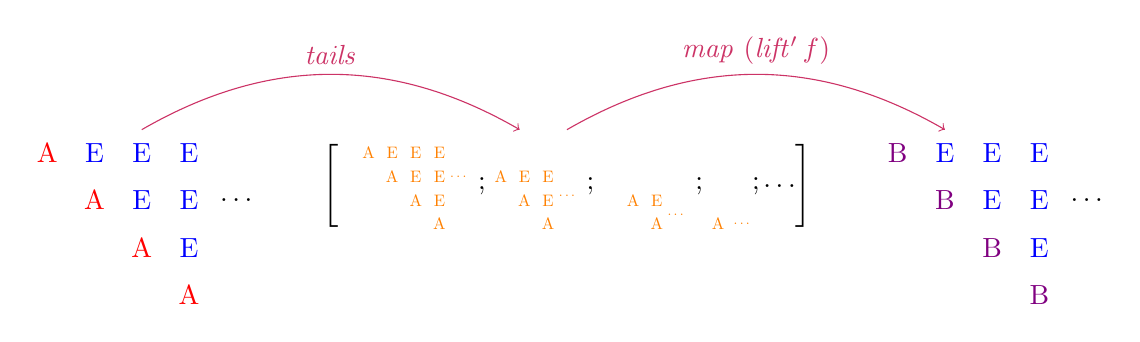
\begin{tikzpicture}[scale = 0.6]
    
    \foreach \y in {0,...,2}
    {\foreach \x in {\y,...,2}
      \draw (\x+1, -\y) node[color=blue]{E} ;
    }
    \foreach \x in {0,...,3} \draw (\x, -\x) node[color=red]{A} ;
    \draw(4,-1) node{$\ldots$};

    \draw (6, -0.7) node{$\Bigg [$} ;
    \draw (16, -0.7) node{$\Bigg ]$} ;
    
    \foreach \x in {0,...,2} 
    {
      
      \foreach \b in {0,...,\x}
      {\foreach \a in {0,...,\b}
        \draw (2*2.8-2.8*\x+7.3+\b*0.5, -\a*0.5-1+\x*0.5) node[color=orange,scale=0.6]{E} ;
      }
      \foreach \a in {\x,...,3} {
        \draw (2.3*\x+6.8+\a*0.5, -\a*0.5) node[color=orange,scale=0.6]{A} ;
      }
      \draw(2.3*\x+8.7,-0.5-\x*0.4) node[color=orange,
      scale=0.5]{$\ldots$};
      \draw(2.3*\x+9.2,-0.7) node{;};
    }
    \draw(14.2,-1.5) node[color=orange, scale=0.6]{A};
    \draw(14.7,-1.5) node[color=orange, scale=0.5]{$\ldots$};
    \draw(15,-0.7) node{;};
    \draw(15.5,-0.7) node{$\ldots$};

    \foreach \y in {0,...,2}
    {\foreach \x in {\y,...,2}
      \draw (\x+19, -\y) node[color=blue]{E} ;
    }
    \foreach \x in {0,...,3} \draw (\x+18, -\x) node[color=violet]{B} ;
    \draw(22,-1) node{$\ldots$};

    \draw[->,color = purple!80] (2,0.5) to [bend left] node[auto,
    swap, above]{$\tls$} (10,0.5) ; 
    \draw[->,color = purple!80] (11,0.5) to [bend left] node[auto,
    swap, above]{$\map~(\liftS\,f)$} (19,0.5) ; 

  \end{tikzpicture}
  \caption{Another definition of redecoration}
  \label{fig:redecS'}
\end{figure}

Thus, we define a new version of the redecoration operation as
follows:
\begin{definition}[$\redecSS : \forall A\forall B.\,(\TriS\,A \to B) \to
  \TriS\,A \to \TriS\,B$]
  $$\redecSS\,f\,t := \map\,(\liftS\,f)\,(\tls\,t)$$
\end{definition}
\noindent
One can then easily show that this operation is equivalent to the
previous one: 
\begin{lemma}
  $\forall A\forall B\forall (f: \TriS\,A \to B)\forall (t:
  \TriS\,A).\, \redecS\,f\,t \EqSt \redecSS\,f\,t$
\end{lemma}
The proof is a straightforward coinduction. 

It is interesting to note that here, we do not need the bisimulation
relation defined on \TriS{}. We can directly use the standard relation
on \Str{}, \EqSt{}. This should not be surprising. Indeed, here we
only really manipulate streams. Those streams are made of pairs and we
only manipulate the finite part of each pair (the first element). The
second one is only a copy. Therefore the relation \bisimS{} would be
artificial here. 

Let's continue abstracting and define \redecSG{} as follows:
\begin{definition}[$\redecSG: \forall A\forall B.\,(\Str\,A \to B) \to
  \Str\,A \to \Str\,B$]
  $$\redecSG\,f\,s :=  \map\,f\,(\tls\,s)$$
\end{definition}
\noindent
As we remarked previously, \tls{} has the signature of a
comultiplication for a comonad (in the triple format \cite{maclane}) based on \Str{},
and it is well known that \map{} is the functor (on morphisms) for
\Str{}. Therefore, \redecSG{} becomes the cobind operation of this
comonad, generically. We do not develop this piece of constructive
category theory here, but only state the result for this instance:
\begin{lemma}\label{lemma:StrComonad}
  The type transformation \Str{}, the projection function \hd{} and
  \redecSG{} form a constructive comonad with respect to \EqSt{}.
\end{lemma}

This section is inspired by Adriano
\cite{haskellList:redecorationAnswer}
who suggested 
a redecoration function for Haskell lists just
in this form. More precisely, a function \texttt{slide :: ([a] -> b) -> [a] ->
  [b]} was defined by \texttt{slide f = map f.tails}. Note that Haskell
lists can be finite and infinite, thus this definition captured
streams as well.

The function \redecSS{} is an instance of \redecSG{}, i.\,e.,
the following lemma is trivial: 
\begin{lemma}
  $\forall A\forall B\forall(f:\TriS\,A\to B)(t:\TriS\,A).\, \redecSS\,f\,t = \redecSG\,(\liftS\,f)\,t$
\end{lemma}
\noindent
Therefore, it is natural to show the three laws of comonads for
\redecSS{} and the proofs are much simplified by the use of
\redecSG{}. In particular, we can show a kind of commutativity of $\liftS$ with
\redecSS{}. 

\begin{lemma}
  The type transformation \TriS{}, the projection function \topS{}
  and \redecSS{} form a constructive comonad with respect to \EqSt{}
  (more precisely, the equivalence relation is
  $\EqSt_{A\times\Str\,E}$ for every $A$).
\end{lemma}
\begin{remark}
  Through the functions \tSR{} and \fSR{}, one can then transfer this
  comonad structure back to \Tri{}.  Since \rlem{redecS_redec} and
  \rlem{redec_redecS} require compatibility of $f$ with bisimilarity,
  this will not even give a constructive weak comonad, but the first
  and third law have to be relativized to compatible $f$'s as
  well. Still, this does not seem a problematic constraint. Anyway,
  \rlem{TriWComonad} has been proved independently of streams.
\end{remark}


%%% Local Variables:
%%% mode: latex
%%% TeX-master: "coredec"
%%% End:

\section{Conclusion}

In this paper we have presented various verifications of the
redecoration algorithm for infinite triangles. We have first dualized
directly the representation for finite triangles by a nested inductive
datatype to obtain a nested coinductive datatype. In both cases, the
triangles are visualized by their columns. We have implemented the
corresponding redecoration algorithm \redec{} (already available \cite{grossestcspaper} in
higher-order parametric polymorphism) and
shown that we (only) obtained a constructive weak comonad (because of
the compatibility hypothesis required). In this part, the redecoration
algorithm, although deduced directly from the finite case, is quite
tricky to manipulate because of the cutting and lifting it requires.

We then noticed that we could also consider
the triangles by their rows, representing this time the triangles by
purely coinductive datatypes, \TriS{}, where we only took advantage of the
existing type of streams (\Str). This new visualization allowed us to
define -- keeping the same algorithmic idea as before -- a function of
redecoration \redecS{} already simpler than \redec{} and equivalent to
it, modulo compatibility. But taking advantage of this
representation by streams, we can simplify again the redecoration algorithm,
using only standard functions on streams. This new function
\redecSS{} is fully equivalent to \redecS{}. Generalizing again, we
get nearly for free the cobind of the comonad \Str{}, \redecSG{}. This
finally allows us to prove the three comonad laws for \redecSS{}. 

In short, we have shown that the redecoration function, which is a
quite subtle operation if we translate it directly from the finite
triangles, reduces to something very basic in the completely infinite
(i.\,e., in both directions) view of the infinite
triangles. 
In this case, it is much easier to work with only infinite elements
than with partially finite ones in the sense of consisting of
infinitely many finitely presented columns. In fact, the stream
representation is even easier to manipulate than the representation of
finite triangles, and the comonad laws even hold with less
restrictions due to constructivity. 

Notice that the row-based view would 
not have given new insights for finite triangles. Indeed, as they are
symmetric, we would have obtained exactly the same representation as
for the column-based approach, only perceived with interchanged roles
of rows and columns.

As a final remark on the Coq side, the improved support for setoid
rewriting and the class mechanism \cite{DBLP:conf/tphol/SozeauO08} has
shown to be of great help for the formalization and verification
decribed in this paper.



%%% Local Variables:
%%% mode: latex
%%% TeX-master: "coredec"
%%% End:


%\bibliography{coredec}

\begin{thebibliography}{10}

\bibitem{grossestcspaper}
Andreas Abel, Ralph Matthes, and Tarmo Uustalu.
\newblock Iteration and coiteration schemes for higher-order and nested
  datatypes.
\newblock {\em Theoretical Computer Science}, 333(1--2):3--66, 2005.

\bibitem{haskellList:redecorationAnswer}
Jorge Adriano.
\newblock Answer to {M}arkus {S}chnell's message \texttt{slide: useful
  function?}
\newblock {Haskell Mailing List}, November 2002.

\bibitem{coqart}
Yves Bertot and Pierre Cast{\'e}ran.
\newblock {\em Interactive Theorem Proving and Program Development.
  {C}oq'{A}rt: The Calculus of Inductive Constructions}.
\newblock Texts in Theoretical Computer Science. Springer Verlag, 2004.

\bibitem{birdmeertens}
Richard Bird and Lambert Meertens.
\newblock Nested datatypes.
\newblock In Johan Jeuring, editor, {\em Mathematics of {P}rogram
  {C}onstruction, {MPC}'98, Proceedings}, volume 1422 of {\em Lecture Notes in
  Computer Science}, pages 52--67. Springer Verlag, 1998.

\bibitem{gfolds}
Richard Bird and Ross Paterson.
\newblock Generalised folds for nested datatypes.
\newblock {\em {F}ormal {A}spects of {C}omputing}, 11(2):200--222, 1999.

\bibitem{dan}
Nils~Anders Danielsson.
\newblock Beating the productivity checker using embedded languages.
\newblock In Ana Bove, Ekaterina Komendantskaya, and Milad Niqui, editors, {\em
  PAR}, volume~43 of {\em EPTCS}, pages 29--48, 2010.

\bibitem{daal}
Nils~Anders Danielsson and Thorsten Altenkirch.
\newblock Subtyping, declaratively.
\newblock In Claude Bolduc, Jules Desharnais, and B{\'e}chir Ktari, editors,
  {\em Mathematics of Program Construction}, volume 6120 of {\em Lecture Notes
  in Computer Science}, pages 100--118. Springer, 2010.

\bibitem{maclane}
Saunders {Mac Lane}.
\newblock {\em Categories for the Working Mathematician}, volume~5 of {\em
  Graduate Texts in Mathematics}.
\newblock Springer Verlag, second edition, 1998.

\bibitem{TYPES11code}
Ralph Matthes and Celia Picard.
\newblock Formalization in {C}oq for this article, 2012.
\newblock \url{www.irit.fr/~Celia.Picard/Coq/Redecoration/}.

\bibitem{types07}
Ralph Matthes and Martin Strecker.
\newblock Verification of the redecoration algorithm for triangular matrices.
\newblock In Furio Honsell, Marino Miculan, and Ivan Scagnetto, editors, {\em
  Types for Proofs and Programs, International Conference, TYPES 2007, Revised
  Selected Papers}, volume 4941 of {\em Lecture Notes in Computer Science},
  pages 125--141. Springer Verlag, 2008.

\bibitem{theseCP}
Celia Picard.
\newblock {\em Représentation coinductive des graphes}.
\newblock PhD thesis, Université de Toulouse, 2012.

\bibitem{DBLP:conf/tphol/SozeauO08}
Matthieu Sozeau and Nicolas Oury.
\newblock First-class type classes.
\newblock In Otmane~A\"{\i}t Mohamed, C{\'e}sar Mu{\~n}oz, and Sofi{\`e}ne
  Tahar, editors, {\em TPHOLs}, volume 5170 of {\em Lecture Notes in Computer
  Science}, pages 278--293. Springer, 2008.

\bibitem{MC}
{T}he {C}oq~{D}evelopment {T}eam.
\newblock The {C}oq {P}roof {A}ssistant {R}eference {M}anual.
\newblock INRIA.

\bibitem{DBLP:conf/sfp/UustaluV01}
Tarmo Uustalu and Varmo Vene.
\newblock The dual of substitution is redecoration.
\newblock In Kevin Hammond and Sharon Curtis, editors, {\em Scottish Functional
  Programming Workshop}, volume~3 of {\em Trends in Functional Programming},
  pages 99--110. Intellect, 2001.

\end{thebibliography}


\end{document}
